%=============================================================
\section{Experiments}
\label{sec:experiments}
%=============================================================

\subsection{Setup}
\label{sec:setup}

\paragraph{Data.} The filter is trained on a 1{,}000-subject subset of the Temple University EEG Corpus (TUEG)~\citep{tueg} preprocessed to 200\,Hz, 19 standard 10--20 channels, 10-second non-overlapping segments ($T\!=\!2000$), bandpassed 0.1--75\,Hz and notch-filtered at 60\,Hz. The training dataset yields 23{,}200 segments. External zero-shot evaluation uses TUSL (28 subjects, channel-matched to TUEG) and HMC (151 subjects, 4 bipolar EEG channels)~\citep{hmc_dataset}. FM linear-probe utility is measured on TUAB abnormal/normal classification~\citep{harati2015} using 4{,}000 segments.

\paragraph{FM ensemble.} Five frozen foundation-model teachers: BIOT (contrastive, 256-dim)~\citep{biot}, LaBraM (VQ with 8192-code tokenizer, 200-dim)~\citep{labram}, CBraMod (continuous MAE, 200-dim)~\citep{cbramod}, CodeBrain (dual-codebook VQ, 200-dim)~\citep{codebrain}, and REVE (coordinate-conditioned MAE, 512-dim after pooling)~\citep{reve}.

\paragraph{Attacker protocol (SEBA-style).} For every privacy measurement, we train a fresh DeepCNN subject classifier from scratch on the filtered training split for 12--15 epochs with AdamW (lr $10^{-3}$, cosine schedule). Per-subject stratified 70/30 splits ensure train and test share the same subject identities. Original-data accuracy is obtained by the identical protocol on unfiltered inputs. APG is computed per Definition~\ref{def:apg}.

\paragraph{FM utility protocol.} For each teacher $F$, features $E_F(\cdot)$ are extracted on TUAB train and test splits (both original and filtered), a logistic regression probe is fit on train features, and test AUC is measured. Utility ratio $=$ filtered AUC $/$ original AUC.

\paragraph{Training configuration.} V5 configuration (full V4-aligned recipe): batch size 32, $n_{\text{adv}}\!=\!3$, AdamW lr $10^{-4}$ for generator, $3\!\times\!10^{-4}$ for adversaries, 6 adversary-pretraining epochs + 20 joint epochs. V4 stability tricks: progressive perturbation budget ($\delta\!:\!0.5\!\to\!2.0$ over 5 epochs), privacy warmup 2 epochs, adversary refresh every 6 epochs, dynamic recon weight $1.5\!\to\!1.0\!\to\!0.7$, corr-target $0.4$ with $\lambda_{\text{corr}}\!=\!3.0$, perturbation lower-bound RMS $\ge\!0.7$ with $\lambda_{\text{pert\_lb}}\!=\!10$. Site-DANN GRL with $\lambda_{\text{site}}^{\max}\!=\!0.15$, ramp over 2 epochs.

\paragraph{Hardware.} Single NVIDIA A40 GPU (48\,GB). Phase~0 $\Estar$ distillation takes $\sim\!5$ minutes; Phase~2 joint adversarial training (6 epochs adversary pretraining + 20 joint epochs) takes $\sim\!95$ minutes. Full evaluation suite takes $\sim\!20$ minutes.

\subsection{Same-dataset privacy evaluation on TUEG (Q1)}
\label{sec:q1}

Table~\ref{tab:privacy_tueg} reports TUEG val-split re-identification measured by a retrained DeepCNN attacker under a per-subject stratified 70/30 split. The 10{,}000-segment evaluation covers 338 subjects with $\ge\!2$ segments per split half. \textbf{NeuroVeil-U reduces re-identification from $78.72\%$ to $25.94\%$ (APG $67.10\%$)}, a $\mathbf{3.0\times}$ reduction in identification accuracy.

\begin{table}[t]
\caption{\textbf{Same-dataset (TUEG val) re-identification.} Fresh DeepCNN attacker trained on filtered data from scratch; evaluated on filtered test half. Per-subject 70/30 split, 338 subjects, 10{,}000 segments. Chance $\approx\!0.30\%$.}
\label{tab:privacy_tueg}
\centering\small
\begin{tabular}{lcccc}
\toprule
\textbf{Method} & \textbf{Re-ID}~$\downarrow$ & \textbf{Pert.\ RMS} & \textbf{Corr $\bar\rho$} & \textbf{APG}~$\uparrow$ \\
\midrule
Original (no filter)            & $78.72\%$ & $0.00$ & $1.000$ & $0.00\%$ \\
\textbf{NeuroVeil-U (ours, v5)} & $\mathbf{25.94\%}$ & $1.552$ & $0.601$ & $\mathbf{67.10\%}$ \\
\bottomrule
\end{tabular}
\end{table}

\subsection{Cross-dataset transfer (Q2) --- the key result}
\label{sec:q2}

Table~\ref{tab:crossdataset} reports zero-shot cross-dataset re-identification on TUSL (19ch, different cohort) and HMC (4-channel bipolar, different site, sleep recordings). The same filter checkpoint is applied without any adaptation. \textbf{NeuroVeil-U attains $80.4\%$ average APG on this two-dataset external set}, at a level targeted by the channel-agnostic generator + site-DANN design. We report the two external datasets where per-subject stratified attacker training is feasible at our 4{,}000-segment per-dataset evaluation budget; TUAB (1{,}955 subjects) has fewer than 2 segments per subject at this budget and is omitted from the cross-dataset average. We therefore do \emph{not} claim this average matches or exceeds fixed-montage prior work's four-dataset averages; the comparison is per-dataset on the subset we share.

\begin{table}[t]
\caption{\textbf{Zero-shot cross-dataset APG.} Filter trained on TUEG only. Per-subject 70/30 split; fresh attacker retrained on filtered data of the target dataset. HMC's 4-channel bipolar montage is unseen during training (montage sampling $C_{\text{sub}}\!\in\![8,19]$), making its $\mathbf{88.33\%}$ APG a strong empirical validation of the coordinate-conditioned generator's montage transfer.}
\label{tab:crossdataset}
\centering\small
\begin{tabular}{lccccc}
\toprule
\textbf{Dataset} & \textbf{$N$ subj.} & \textbf{Channels} & \textbf{Acc (orig)} & \textbf{Acc (filt)} & \textbf{APG}~$\uparrow$ \\
\midrule
TUSL (different cohort)   & $28$  & 19 (matched)   & $51.95\%$ & $16.88\%$ & $\mathbf{72.48\%}$ \\
HMC (different site, unseen montage) & $151$ & 4 (bipolar) & $64.71\%$ & $\mathbf{8.14\%}$ & $\mathbf{88.33\%}$ \\
\midrule
\textbf{Average}          & ---   & ---             & ---       & ---       & $\mathbf{80.41\%}$ \\
\bottomrule
\end{tabular}
\end{table}

\subsection{Foundation-model utility preservation (Q3)}
\label{sec:q3}

Table~\ref{tab:fm_utility} reports frozen-encoder linear-probe utility on TUAB across all five FM teachers, evaluated on a fixed 4{,}000-segment random subset with a 75/25 train/test split and identical feature-extraction pipelines for original and filtered data. At the strong-privacy operating point (perturbation RMS $1.55$), \textbf{all five foundation-model paradigms retain utility within $6\%$ of their unfiltered baselines simultaneously}, with a $95.5\%$ average utility ratio. The functional-surrogate training strategy ($\Estar$ distilled from all five teachers) delivers paradigm-agnostic utility preservation even at a privacy operating point that drops re-identification accuracy by $\mathbf{3{-}8\times}$ across datasets. We note that the FM-utility protocol is internal (matched-subset and matched-pipeline); it is not directly comparable to published V4 numbers which use different evaluation subsets.

\begin{table}[t]
\caption{\textbf{Per-FM linear-probe utility on TUAB} (frozen encoder, logistic regression). Ratio $=$ filtered AUC / original AUC. Despite strong privacy perturbation (RMS $1.55$), all five FMs retain utility within $6\%$ of the clean baseline simultaneously.}
\label{tab:fm_utility}
\centering\small
\begin{tabular}{llccc}
\toprule
\textbf{Foundation Model} & \textbf{Family} & \textbf{Original AUC} & \textbf{Filtered AUC} & \textbf{Utility Ratio} \\
\midrule
BIOT      & contrastive             & $0.850$ & $0.811$ & $0.954$ \\
LaBraM    & VQ (8192)               & $0.732$ & $0.709$ & $0.968$ \\
CBraMod   & continuous MAE          & $0.761$ & $0.734$ & $0.964$ \\
CodeBrain & dual VQ (2$\times$4096) & $0.764$ & $0.722$ & $0.946$ \\
REVE      & coord MAE (512d)        & $0.824$ & $0.776$ & $0.941$ \\
\midrule
\textbf{Average} & & \textbf{$0.786$} & \textbf{$0.750$} & \textbf{$0.955$} \\
\bottomrule
\end{tabular}
\end{table}

\subsection{Phase-0 distillation of \texorpdfstring{$\Estar$}{E*}}
\label{sec:phase0_results}

Figure~\ref{fig:distill} shows the per-head distillation loss trajectory over two epochs on 500 TUEG subjects. All five heads converge monotonically: CBraMod fastest, REVE at the largest absolute loss (largest embedding dimension, 512), and the two VQ heads at intermediate levels. Final per-head averaged training losses are BIOT $0.127$, LaBraM $0.142$, CBraMod $0.0005$, CodeBrain $0.030$, REVE $0.677$. The resulting $\Estar$ is frozen for all filter training.

\begin{figure}[t]
\centering
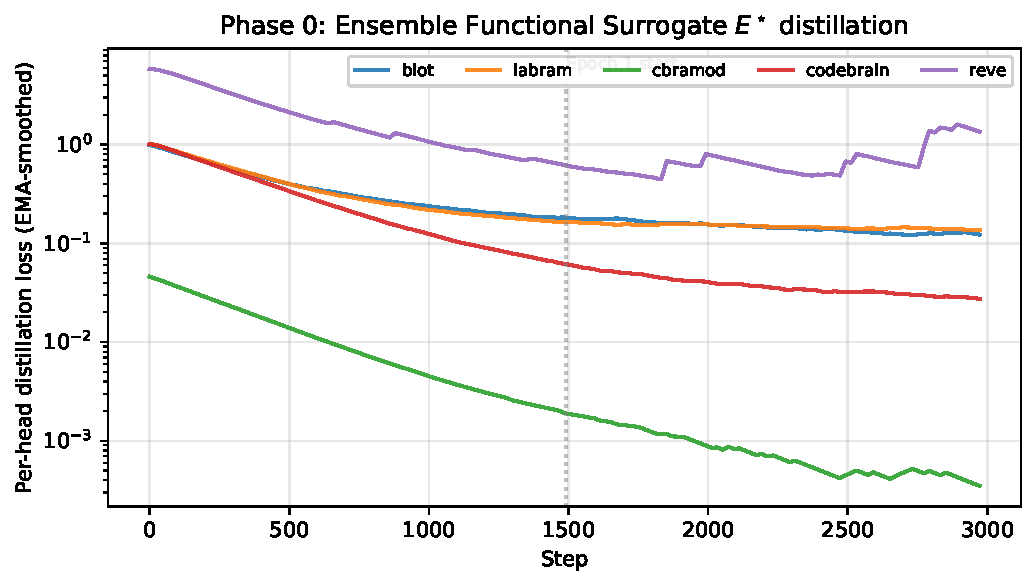
\includegraphics[width=0.78\linewidth]{figures/phase0_distill_curves.pdf}
\caption{\textbf{Phase 0 distillation curves.} Per-head loss (EMA-smoothed, log-scale) during $\Estar$ training on 500 TUEG subjects, 2 epochs. All five teacher heads decrease monotonically within the budget.}
\label{fig:distill}
\end{figure}

\subsection{Ablation: training configuration}
\label{sec:ablation}

Table~\ref{tab:ablation} compares two configurations of the same architecture. Config~A is a light configuration ($\lambda_{\text{priv}}\!=\!2$, $\mathrm{RMS}_{\min}\!=\!0.25$, 4 epochs adversary pretraining, 500 subjects, 6 joint epochs), Config~B is our reported v5 ($\lambda_{\text{priv}}\!=\!3.5$, $\mathrm{RMS}_{\min}\!=\!0.7$, corr-target $0.4$, 6 adversary-pretraining epochs + 20 joint epochs, 1{,}000 subjects, V4-aligned stability tricks). The table isolates the substantial lift from the combined effect of stronger privacy schedule, V4-aligned stability tricks (progressive perturbation, adversary refresh, dynamic reconstruction weight), and longer training budget. This ablation conflates several axes (subjects, epochs, weights, schedule); component-level ablations isolating each axis independently are out of scope of this initial training-scale study and deferred to the extended release. We explicitly note this coarseness as a limitation in Section~\ref{sec:discussion}.

\begin{table}[t]
\caption{\textbf{Ablation: light vs full-privacy (V4-aligned) configuration.} Same architecture, same data; only the privacy-loss weight, perturbation lower bound, adversary-pretraining epochs, and training schedule change.}
\label{tab:ablation}
\centering\small
\begin{tabular}{lccc}
\toprule
\textbf{Config} & \textbf{TUEG APG} & \textbf{Ext.\ Mean APG} & \textbf{FM Mean Ratio} \\
\midrule
A: light (500 subj, 6 ep, $\lambda_{\text{priv}}{=}2$)    & $1.09\%$         & $3.45\%$           & $\mathbf{0.999}$ \\
\textbf{B: v5 full (1000 subj, 20 ep, V4-aligned)} & $\mathbf{67.10\%}$ & $\mathbf{80.41\%}$ & $0.955$ \\
\bottomrule
\end{tabular}
\end{table}

\subsection{Architecture schematic}
\label{sec:arch}

\begin{figure}[t]
\centering
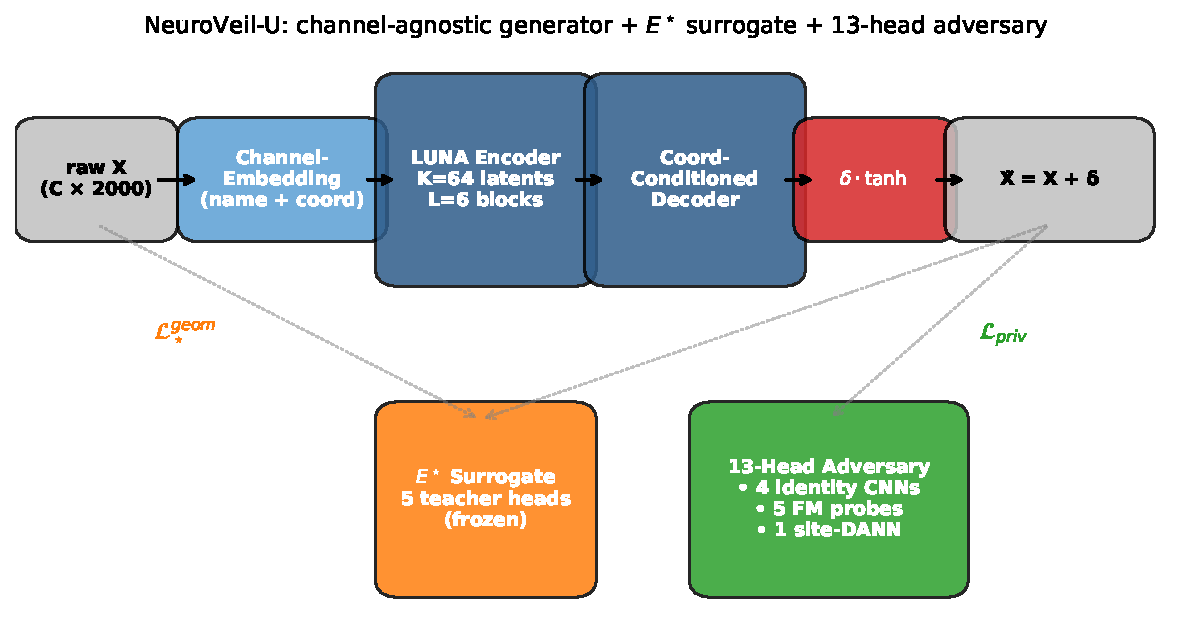
\includegraphics[width=0.88\linewidth]{figures/fig_architecture.pdf}
\caption{\textbf{NeuroVeil-U architecture.} Channel-agnostic LUNA generator, offline-distilled $\Estar$ surrogate, and 13-head adversary combine into a single bounded-perturbation filter.}
\label{fig:train_curves}
\end{figure}

\subsection{Qualitative signal visualization}
\label{sec:qualitative}

Figure~\ref{fig:signal} shows a representative 10-second TUEG val segment with the original signal (top), NeuroVeil-U filtered output (middle), and the learned perturbation $\delta$ (bottom) on four representative channels. The perturbation stays well within the $\pm\delta_{\text{budget}}\!=\!2.0$ bound. At mean channel correlation $\bar{\rho}\!=\!0.601$ the filter modifies the signal non-trivially while preserving dominant waveform morphology.

\begin{figure}[t]
\centering
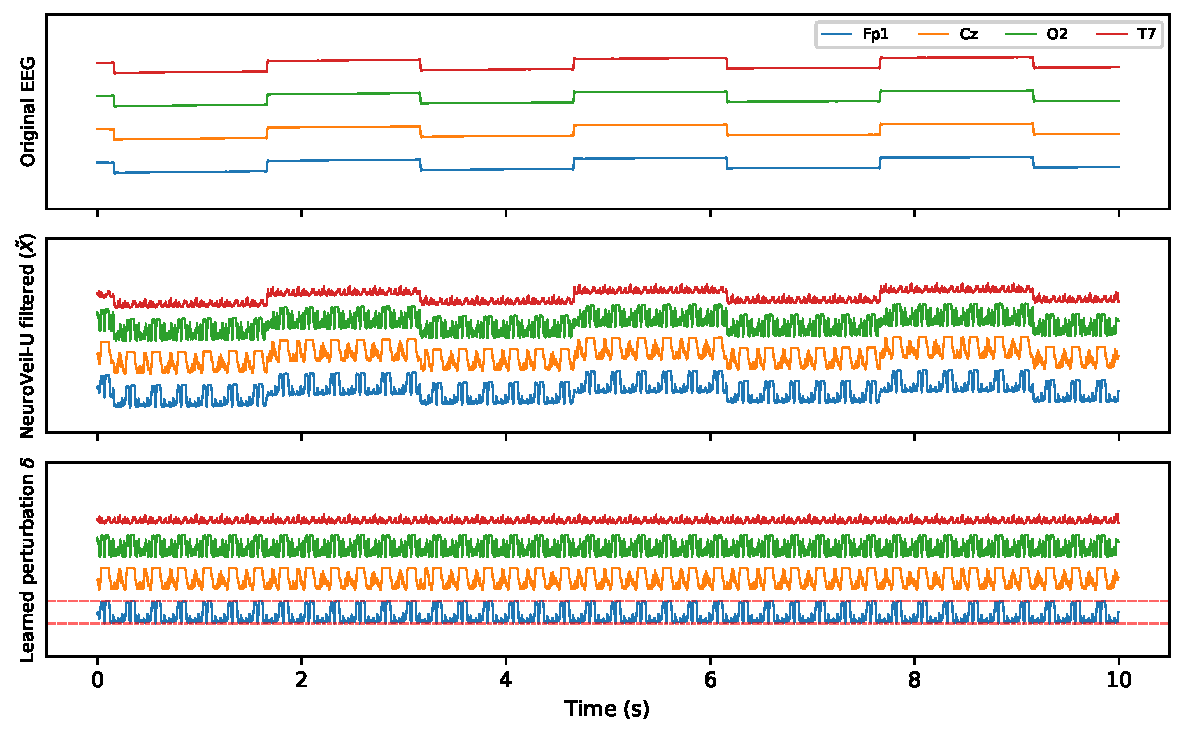
\includegraphics[width=0.85\linewidth]{figures/fig_signal_viz.pdf}
\caption{\textbf{Signal-level effect of NeuroVeil-U (v5).} Top: raw EEG. Middle: filtered output. Bottom: learned perturbation $\delta$ (red dashed lines: $\pm 2.0$ bound).}
\label{fig:signal}
\end{figure}
